\documentclass[tikz, border=8pt]{standalone}
\usepackage{amsmath}
\usepackage{tikz}
\usetikzlibrary{arrows.meta, calc, shadings, positioning,
                decorations.pathmorphing, shapes.geometric}

\begin{document}
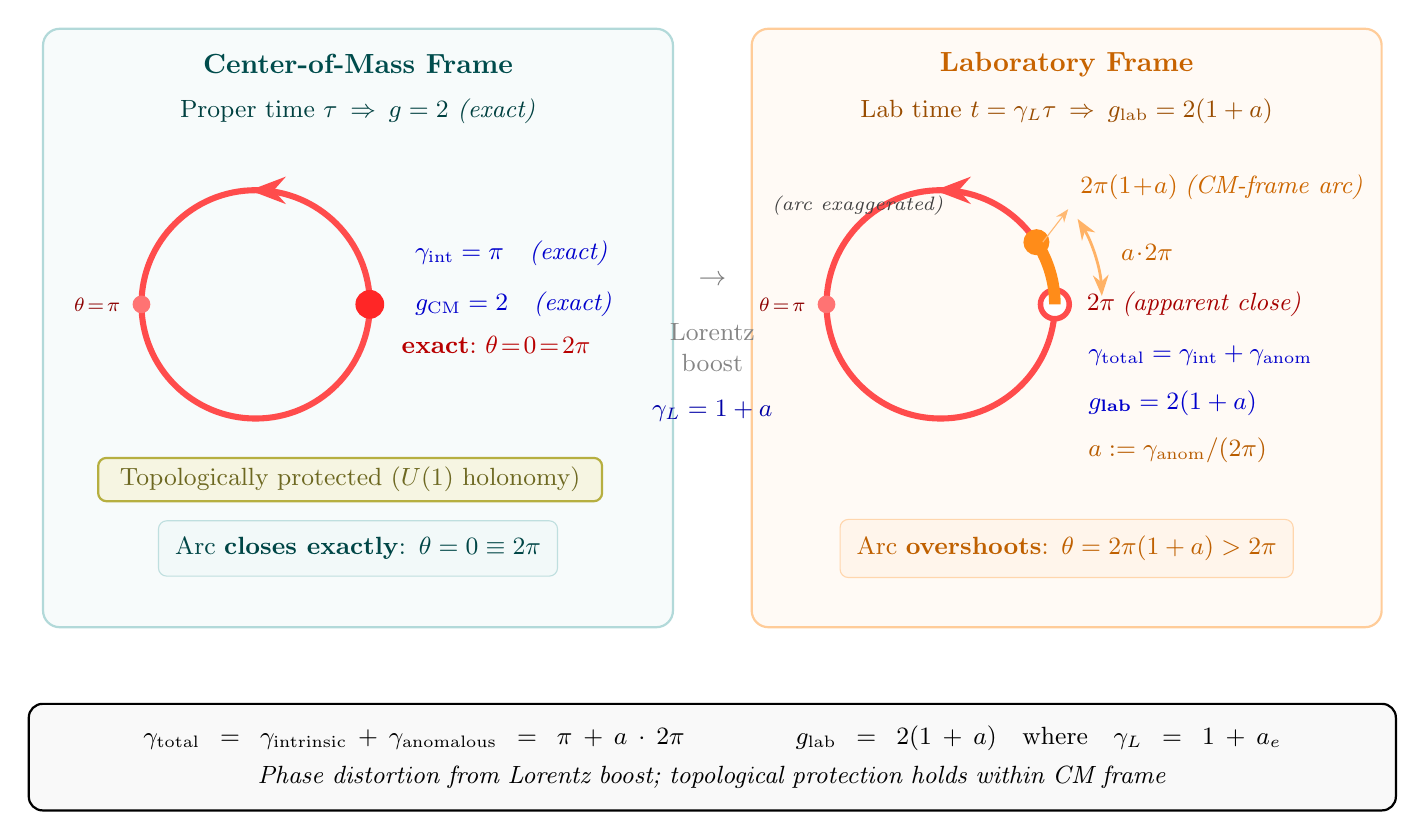
\begin{tikzpicture}[>=Stealth, font=\small]

%%====================================================
%% LEFT BOX — CENTER-OF-MASS FRAME
%% x in [-8.5, -0.5],  y in [-3.2, 4.4]
%%====================================================
\draw[thick, rounded corners=6pt, fill=teal!3, draw=teal!30]
  (-8.5, -3.2) rectangle (-0.5, 4.4);

%% Title + subtitle
\node[font=\normalsize\bfseries, teal!60!black] at (-4.5, 3.95)
  {Center-of-Mass Frame};
\node[font=\small, teal!50!black] at (-4.5, 3.35)
  {Proper time $\tau$\enspace $\Rightarrow$\enspace $g = 2$ \textit{(exact)}};

%% Circle: center (-5.8, 0.9), radius 1.45cm — full CCW red orbit
\draw[red!70, line width=2.2pt] (-4.35, 0.9) arc (0:360:1.45cm);
%% CCW arrow at top
\draw[red!70, ->, line width=2.2pt]
  ({-5.8+1.45*cos(87)}, {0.9+1.45*sin(87)}) --
  ({-5.8+1.45*cos(93)}, {0.9+1.45*sin(93)});
%% θ=π dot (leftmost)
\filldraw[red!55] (-7.25, 0.9) circle (3.0pt);
\node[left=4pt, font=\scriptsize, red!55!black] at (-7.25, 0.9) {$\theta\!=\!\pi$};
%% Exact closure: FILLED dot at θ=0=2π
\filldraw[red!85] (-4.35, 0.9) circle (5.0pt);
\node[anchor=north west, xshift=8pt, yshift=-8pt, font=\small, red!72!black] at (-4.35, 0.9)
  {\textbf{exact}:\ $\theta\!=\!0\!=\!2\pi$};

%% Annotations — right side of circle (x > -4.1)
\node[anchor=west, font=\small, blue!80!black] at (-3.9, 1.55)
  {$\gamma_{\text{int}} = \pi$\quad\textit{(exact)}};
\node[anchor=west, font=\small, blue!80!black] at (-3.9, 0.90)
  {$g_{\text{CM}} = 2$\quad\textit{(exact)}};

%% Topological protection badge — below circle
\draw[olive!65, rounded corners=3pt, fill=olive!8, thick]
  (-7.8, -1.60) rectangle (-1.4, -1.05);
\node[font=\small, olive!70!black] at (-4.6, -1.32)
  {Topologically protected ($U(1)$ holonomy)};

%% Key result box
\node[draw=teal!25, rounded corners=3pt, fill=teal!5,
  font=\small, text=teal!55!black, inner sep=6pt] at (-4.5, -2.20)
  {Arc \textbf{closes exactly}:\enspace $\theta = 0 \equiv 2\pi$};

%%====================================================
%% RIGHT BOX — LABORATORY FRAME
%% x in [0.5, 8.5],  y in [-3.2, 4.4]
%%====================================================
\draw[thick, rounded corners=6pt, fill=orange!4, draw=orange!40]
  (0.5, -3.2) rectangle (8.5, 4.4);

%% Title + subtitle
\node[font=\normalsize\bfseries, orange!78!black] at (4.5, 3.95)
  {Laboratory Frame};
\node[font=\small, orange!60!black] at (4.5, 3.35)
  {Lab time $t = \gamma_L\tau$\enspace $\Rightarrow$\enspace $g_{\text{lab}} = 2(1+a)$};

%% Circle: center (2.9, 0.9), radius 1.45cm
\draw[red!70, line width=2.2pt] (4.35, 0.9) arc (0:360:1.45cm);
%% CCW arrow at top
\draw[red!70, ->, line width=2.2pt]
  ({2.9+1.45*cos(87)}, {0.9+1.45*sin(87)}) --
  ({2.9+1.45*cos(93)}, {0.9+1.45*sin(93)});
%% θ=π dot (leftmost)
\filldraw[red!55] (1.45, 0.9) circle (3.0pt);
\node[left=4pt, font=\scriptsize, red!55!black] at (1.45, 0.9) {$\theta\!=\!\pi$};
%% Open dot at θ=0 (apparent close, lab frame)
\filldraw[white] (4.35, 0.9) circle (5.2pt);
\draw[red!70, line width=2.0pt] (4.35, 0.9) circle (5.2pt);
\node[anchor=west, xshift=8pt, font=\small, red!65!black] at (4.35, 0.9)
  {$2\pi$\;\textit{(apparent close)}};
%% Orange arc: excess a·2π (exaggerated, 0→33°)
\draw[orange!90, line width=4.2pt] (4.35, 0.9) arc (0:33:1.45cm);
\filldraw[orange!90]
  ({2.9+1.45*cos(33)},{0.9+1.45*sin(33)}) circle (4.5pt);
%% Leader from orange dot to label
\node[anchor=south west, font=\small, orange!80!black]
  (cmLabel) at (4.55, {0.9+1.45*sin(33)+0.42})
  {$2\pi(1\!+\!a)$\;\textit{(CM-frame arc)}};
\draw[orange!55, thin, ->]
  ({2.9+1.45*cos(33)+0.08},{0.9+1.45*sin(33)}) -- (4.52, {0.9+1.45*sin(33)+0.42});
%% Double-arrow for gap
\draw[<->, orange!60, line width=1.0pt]
  ({2.9+2.05*cos(3)},{0.9+2.05*sin(3)}) arc (3:32:2.05cm);
\node[font=\small, orange!78!black]
  at ({2.9+2.70*cos(14)},{0.9+2.70*sin(14)}) {$a\!\cdot\!2\pi$};
\node[font=\scriptsize, gray!50!black] at (1.85, 2.15) {\textit{(arc exaggerated)}};

%% Berry phase decomposition — right area
\node[anchor=west, font=\small, blue!80!black] at (4.65, 0.25)
  {$\gamma_{\text{total}} = \gamma_{\text{int}} + \gamma_{\text{anom}}$};
\node[anchor=west, font=\small\bfseries, blue!80!black] at (4.65, -0.35)
  {$g_{\text{lab}} = 2(1+a)$};
\node[anchor=west, font=\small, orange!72!black] at (4.65, -0.95)
  {$a := \gamma_{\text{anom}}/(2\pi)$};

%% Key result box
\node[draw=orange!32, rounded corners=3pt, fill=orange!8,
  font=\small, text=orange!75!black, inner sep=6pt] at (4.5, -2.20)
  {Arc \textbf{overshoots}:\enspace $\theta = 2\pi(1+a) > 2\pi$};

%%====================================================
%% CENTRE — Lorentz boost arrow
%%====================================================
\node[font=\normalsize\bfseries, black!52] at (0, 1.20) {$\rightarrow$};
\node[font=\small, black!48, align=center] at (0, 0.35)
  {Lorentz\\boost};
\node[font=\small, blue!65!black, align=center] at (0, -0.45)
  {$\gamma_L = 1+a$};

%%====================================================
%% BOTTOM STRIP — unifying equation
%%====================================================
\node[draw, thick, rounded corners=5pt, fill=gray!5,
  text width=16.8cm, font=\small, align=center, inner sep=8pt]
  at (0, -4.85) {
  $\gamma_{\text{total}} = \gamma_{\text{intrinsic}} + \gamma_{\text{anomalous}} = \pi + a\cdot 2\pi$
  \qquad\qquad
  $g_{\text{lab}} = 2(1+a)$\quad where\quad $\gamma_L = 1 + a_e$\\[3pt]
  \textit{Phase distortion from Lorentz boost; topological protection holds within CM frame}
};

\end{tikzpicture}
\end{document}